\documentclass[UTF8]{beamer}
\usepackage{hyperref}
\usepackage{outlines}
\usepackage{graphicx}
\usepackage{caption}
\usepackage{subcaption}
\usepackage{algorithm}
\usepackage{algorithmic}
\usepackage{amsmath,amssymb}
\usepackage[T1]{fontenc}
\usepackage{moresize}
\usepackage[english]{babel}
\usepackage{tikz}
\usetikzlibrary{overlay-beamer-styles}

\usepackage{latexsym,xcolor,multicol,booktabs,calligra}
\usepackage{pstricks,listings,stackengine}
\usepackage[table]{xcolor}
\usepackage[dvipsnames]{xcolor}
\usepackage{cancel}

% Ensure English labels
\renewcommand{\figurename}{Figure}
\renewcommand{\algorithmname}{Algorithm}

% Theme (same as your previous)
\usepackage{SHU}

% --- Small helper defs ---
\def\cmd#1{\texttt{\color{red}\footnotesize $\backslash$#1}}
\def\env#1{\texttt{\color{blue}\footnotesize #1}}
\definecolor{deepblue}{rgb}{0,0,0.5}
\definecolor{deepred}{rgb}{0.6,0,0}
\definecolor{deepgreen}{rgb}{0,0.5,0}
\definecolor{halfgray}{gray}{0.55}
\definecolor{nus-orange}{RGB}{239,124,0}
\definecolor{nus-white}{RGB}{255,255,255}
\definecolor{nus-blue}{RGB}{0,61,124}
\definecolor{nus-black}{RGB}{0,0,0}

\newcommand\vscore{\mathsf{VScore}}
\newcommand\Fontvi{\fontsize{6}{7.2}\selectfont}
\newcommand{\ZZ}{\mathbb{Z}}
\newcommand{\NN}{\mathbb{N}}
\newcommand{\q}{$q_\mathrm{ex}$}
\renewcommand{\leq}{\leqslant}
\renewcommand{\geq}{\geqslant}

\lstset{
  basicstyle=\ttfamily\small,
  keywordstyle=\bfseries\color{nus-blue},
  emphstyle=\ttfamily\color{nus-blue},
  stringstyle=\color{deepgreen},
  numbers=left,
  numberstyle=\small\color{halfgray},
  rulesepcolor=\color{nus-orange},
  frame=shadowbox,
}

\author{\href{https://pratik2358.github.io/}{Pratik Karmakar}}
\title{BT5110: Tutorial 4 — Normal Forms}
\institute{
  School of Computing,\\
  National University of Singapore
}
\date{AY25/26 S1}

\begin{document}

\begin{frame}
  \titlepage
  \begin{figure}[htpb]
    \begin{center}
      
\includegraphics[keepaspectratio, scale=0.18]{nus-logo.png}
    \end{center}
  \end{figure}
\end{frame}

\section{Question}
\begin{frame}{Question}
\footnotesize
Your company, Apasaja Private Limited, is commissioned by \emph{Toko Kopi Luwak} to design the relational schema for the management of their coffee beans, drinks, and cafes.\medskip

A coffee bean is fully identified by its unique brand name \emph{or} by the pair (cultivar, region). A drink can be made using a particular coffee bean; the drink name is only unique \emph{per} bean (e.g., ``Espresso'' with bean ``The Waterfall'' or with bean ``La Bella''). We also record the drink price.\medskip

A branch (identified by branch name) may sell zero or more drinks; a drink may be sold by zero or more branches. Each branch records an address, and for each (branch, drink) pair we record the quantity sold.
\medskip

We are given only an abstract schema:
\[
R=\{A,B,C,D,E,F,G,H\}
\]
\[
\Sigma=\{\{A\} \to \{C,E\}, \{A,B\} \to \{D\}, \{F\} \to \{H\}, \{C,E\} \to \{A\},\\
\{B,C,E\} \to \{D\}, \{A,B,F\} \to \{D,G\}, \{B,C,E,F\} \to \{G\}\}.
\]
\end{frame}

\begin{frame}{Question}
\footnotesize
\textbf{1.\ Normal Form}
\begin{itemize}
  \item[(a)] Is $R$ with $\Sigma$ in 3NF?
  \item[(b)] Is $R$ with $\Sigma$ in BCNF?
\end{itemize}
\textbf{2.\ Normalisation}
\begin{itemize}
  \item[(a)] Decompose (synthesise) $R$ with $\Sigma$ into a 3NF decomposition using the lecture algorithm.
  \item[(b)] Is the result lossless?
  \item[(c)] Is the result dependency preserving?
  \item[(d)] Is the result in BCNF?
  \item[(e)] Decompose $R$ with $\Sigma$ into a BCNF decomposition using the lecture algorithm.
  \item[(f)] Is the result lossless?
  \item[(g)] Is the result dependency preserving?
\end{itemize}
\end{frame}

\section{Solutions}

\begin{frame}{1(a).\ Is $R$ with $\Sigma$ in 3NF?}
\footnotesize
\pause
\begin{block}{Criteria for 3NF}
    If $X\to \{A\} \in \Sigma$:
    \begin{itemize}
        \item $X\to \{A\}$ is trivial \alert{or}
        \item $X$ is a superkey \alert{or}
        \item $A$ is a prime attribute
    \end{itemize}
\end{block}
\pause
\textbf{Known keys (from previous tutorial):} $\{A,B,F\}$ and $\{B,C,E,F\}$.\\
\textbf{Prime attributes:} $\{A,B,C,E,F\}$.\\
\pause
Consider $\{A,B\}\to\{D\}$:
\begin{itemize}\itemsep2pt
\pause
  \item Nontrivial.
\pause
  \item $\{A,B\}$ is \emph{not} a superkey.
\pause
  \item $D$ is not a prime attribute.
\end{itemize}
\pause
\[
\Rightarrow\ \ R\text{ with }\Sigma\ \alert{\textbf{is not in 3NF.}}
\]
\end{frame}

\begin{frame}{1(b).\ Is $R$ with $\Sigma$ in BCNF?}
\footnotesize
\begin{columns}
\pause
    \begin{column}{0.5\textwidth}
        \begin{block}{Criteria for 3NF}
    If $X\to \{A\} \in \Sigma$:
    \begin{itemize}
        \item $X\to \{A\}$ is trivial \alert{or}
        \item $X$ is a superkey \alert{or}
        \item $A$ is a prime attribute
    \end{itemize}
\end{block}
    \end{column}
    \pause
    \begin{column}{0.5\textwidth}
        \begin{block}{Criteria for BCNF}
    If $X\to \{A\} \in \Sigma$:
    \begin{itemize}
        \item $X\to \{A\}$ is trivial \alert{or}
        \item $X$ is a superkey
    \end{itemize}
\end{block}
    \end{column}
\end{columns}
\pause
\vspace{0.5cm}
Since not 3NF, cannot be BCNF.\\
A direct violation: $\{A\}\to\{C\}$ is nontrivial and
\[
A^+=\{A,C,E\}\subset R\quad\Rightarrow\quad \{A\}\ \text{is not a superkey}.
\]
So $R$ with $\Sigma$ \textbf{is not in BCNF}.
\end{frame}

\begin{frame}{2(a).\ 3NF synthesis (decomposition)}

\pause
\textbf{Canonical cover:}
$
\{\ \{A\} \to \{C,E\},\ \{F\} \to \{H\},\ \{C,E\} \to \{A\},\ \{B,C,E\} \to \{D\},\ \{B,C,E,F\} \to \{G\}\ \}.
$\\
\pause
\textbf{Candidate keys:}
$\{A,B,F\}, \{B,C,E,F\}$\\
\pause
\textbf{Fragments:}\\
$
R_1 = \{A,C,E\}, \quad R_2 =  \{F,H\},\\
R_3 = \{A,C,E\}, \quad R_4 =  \{B,C,D,E\}, \\
R_5 = \{B,C,E,F,G\}\.
$\\
\pause
\textbf{Remove subsumed/duplicates:}
$R_1$ and $R_3$ are same. So, we remove $R_3$.\\
A key fragment is not needed (the key $\{B,C,E,F\}\subseteq \{B,C,E,F,G\}$ is covered).
\end{frame}

\begin{frame}{2(b).\ Is the result dependency preserving?}
\textbf{Dependency preserving:} Yes, guaranteed by the algorithm (each FD is placed in some fragment, and cover equivalence is preserved).\\
\pause
\alert{Also:}\\
\alert{\textbf{Lossless:} Yes, guaranteed by the 3NF synthesis algorithm.}\medskip
\end{frame}

\begin{frame}{2(c).\ Is the result in BCNF?}
\scriptsize
\begin{columns}
\pause
\hspace{0.2cm}
    \begin{column}{0.23\textwidth}
        $R_1 = \{A,C,E\}\\
        \Sigma_1 = \{\{A\}\to\{C\}, \{A\}\to\{E\},\{C,E\}\to\{A\}\}$\\
        \textbf{Candidate keys:} $\{A\}, \{C,E\}$
    \end{column}
    \pause
    \hspace{-0.35cm}\vline\hspace{0.1cm}
    \begin{column}{0.23\textwidth}
        $R_2 = \{F, H\}\\
        \Sigma_2 = \{\{F\}\to \{H\}\}$\\
        \textbf{Candidate keys:} $\{F\}$
    \end{column}
    \pause
    \hspace{-0.45cm}\vline\hspace{0.15cm}
    \begin{column}{0.23\textwidth}
        $R_4 = \{B,C,D,E\}\\
        \Sigma_4 = \{\{B,C,E\} \to \{D\}\}\\
        \textbf{Candidate keys:} \{B,C,E\}$
    \end{column}
    \pause
    \hspace{-0.3cm}\vline\hspace{0.1cm}
    \begin{column}{0.23\textwidth}
        $R_5 = \{B,C,E,F,G\}\\
        \Sigma_5 = \{\{B,C,E,F\} \to \{G\}\}\\
        \textbf{Candidate keys:} \{B,C,E,F\}$
    \end{column}
\end{columns}
\normalsize
\pause
\vspace{0.5cm}
$\Sigma_1, \Sigma_2, \Sigma_4$ and $\Sigma_5$ are projected dependencies. We obtain these by projecting $\Sigma$ on $R_1, R_2, R_4$ and $R_5$ respectively.\footnote{Dependency projection algorithm: Algorithm~\ref{algorithm:algo}}\\
\pause
\vspace{0.3cm}
$R_1$ with $\Sigma_1$, $R_2$ with $\Sigma_2$, $R_4$ with $\Sigma_4$, and $R_5$ with $\Sigma_5$ satisfy the BCNF criteria individually.
\pause
Thus the result is in BCNF. \alert{(This is not a general case though. There is no guarantee that synthesising a 3NF will yield a BCNF too.)}
\end{frame}

\section{Supplementary}

\begin{frame}{Dependency Projection Algorithm}
\begin{algorithm}[H]
\scriptsize
\caption{Computing FD Projections (closure-based)}
\label{algorithm:algo}
\label{alg:fd-projection-closures}
\begin{algorithmic}[1]
\REQUIRE $G$ : set of functional dependencies on schema $R$
\REQUIRE $R' \subseteq R$ : attribute set to project onto
\ENSURE $G_{R'}$ : projection of $G$ onto $R'$
\STATE $G_{R'} \gets \varnothing$
\FORALL{$Y \subseteq R'$}
    \STATE $T \gets \textsc{Closure}(Y,\; G)$ \hfill// compute $Y^+$ w.r.t.\ $G$
    \STATE $H \gets T \cap X$
    \STATE $G_{R'} \gets G_{R'} \cup \{\, Y \to H \,\}$ \hfill// optionally emit unit FDs: $\{\,Y\to A \mid A \in H\setminus Y\,\}$
\ENDFOR
\STATE \textbf{return} $G_X$
\end{algorithmic}
\end{algorithm}

\end{frame}

\begin{frame}[fragile]{Dependency Projection Example}
\scriptsize
\begin{columns}
  \begin{column}{0.3\textwidth}
    $R=\{A,B,C,D,E\}$\\[0.2cm]
    $\Sigma=\{\ \{A\}\!\to\!\{A,B,C\},\ \{A,B\}\!\to\!\{A\},\ \{B,C\}\!\to\!\{A,D\},\ \{B\}\!\to\!\{A,B\},\ \{C\}\!\to\!\{D\}\ \}$\\[0.2cm]
    $R'=\{A,B,C\}$
  \end{column}
  \begin{column}{0.7\textwidth}
    \tiny
    $\Sigma' \gets \emptyset$\\[2pt]\pause

    \textcolor{blue}{$Y=\{A\}$} \\
    $T=Y^+ \ (\text{w.r.t. }\Sigma)=\{A,B,C,D\}$,\quad $H=T\cap R'=\{A,B,C\}$\\
    $\Sigma' \gets \Sigma' \cup \{\{A\}\to\{A,B,C\}\}$\\[4pt]\pause

    \textcolor{blue}{$Y=\{B\}$} \\
    $T=\{A,B,C,D\}$,\quad $H=\{A,B,C\}$\\
    $\Sigma' \gets \Sigma' \cup \{\{B\}\to\{A,B,C\}\}$\\[4pt]\pause

    \textcolor{blue}{$Y=\{C\}$} \\
    $T=\{C,D\}$,\quad $H=\{C\}$\\
    $\Sigma' \gets \Sigma' \cup \{\{C\}\to\{C\}\}$\\[4pt]\pause

    \textcolor{blue}{$Y=\{A,B\}$} \\
    $T=\{A,B,C,D\}$,\quad $H=\{A,B,C\}$\\
    $\Sigma' \gets \Sigma' \cup \{\{A,B\}\to\{A,B,C\}\}$\\[4pt]\pause

    \textcolor{blue}{$Y=\{A,C\}$} \\
    $T=\{A,B,C,D\}$,\quad $H=\{A,B,C\}$\\
    $\Sigma' \gets \Sigma' \cup \{\{A,C\}\to\{A,B,C\}\}$\\[4pt]\pause

    \textcolor{blue}{$Y=\{B,C\}$} \\
    $T=\{A,B,C,D\}$,\quad $H=\{A,B,C\}$\\
    $\Sigma' \gets \Sigma' \cup \{\{B,C\}\to\{A,B,C\}\}$\\[4pt]\pause

    \textcolor{blue}{$Y=\{A,B,C\}$} \\
    $T=\{A,B,C,D\}$,\quad $H=\{A,B,C\}$\\
    $\Sigma' \gets \Sigma' \cup \{\{A,B,C\}\to\{A,B,C\}\}$
  \end{column}
\end{columns}
\end{frame}

\begin{frame}{Dependency Projection Example (Contd.)}
\textcolor{red}{$\displaystyle
      \Sigma'=\big\{
        \{A\}\!\to\!\{A,B,C\},\
        \{B\}\!\to\!\{A,B,C\},\
        \{C\}\!\to\!\{C\},\
        \{A,B\}\!\to\!\{A,B,C\},\
        \{A,C\}\!\to\!\{A,B,C\},\
        \{B,C\}\!\to\!\{A,B,C\},\
        \{A,B,C\}\!\to\!\{A,B,C\}
      \big\}.
    $}\\
    In the last step, reduce the redundancies from $\Sigma'$:\\
    \textcolor{red}{$\displaystyle
      \Sigma'=\big\{
        \{A\}\!\to\!\{B,C\},\
        \{B\}\!\to\!\{A\}
      \big\}.
    $}\\
    Notice that in this case you could stop after finding the closures of $A$ and $B$ as $\{A\}^+ = R'$ and $\{B\}^+ = R'$, and all other subsets of $R$ contain either $A$ or $B$.
\end{frame}

\section{Overview}
\begin{frame}{Overview}
\begin{center}
    
\includegraphics[width = 1\linewidth]{fd_norm_images/01.png}
\end{center}
\end{frame}

\begin{frame}{Overview}
\begin{center}
    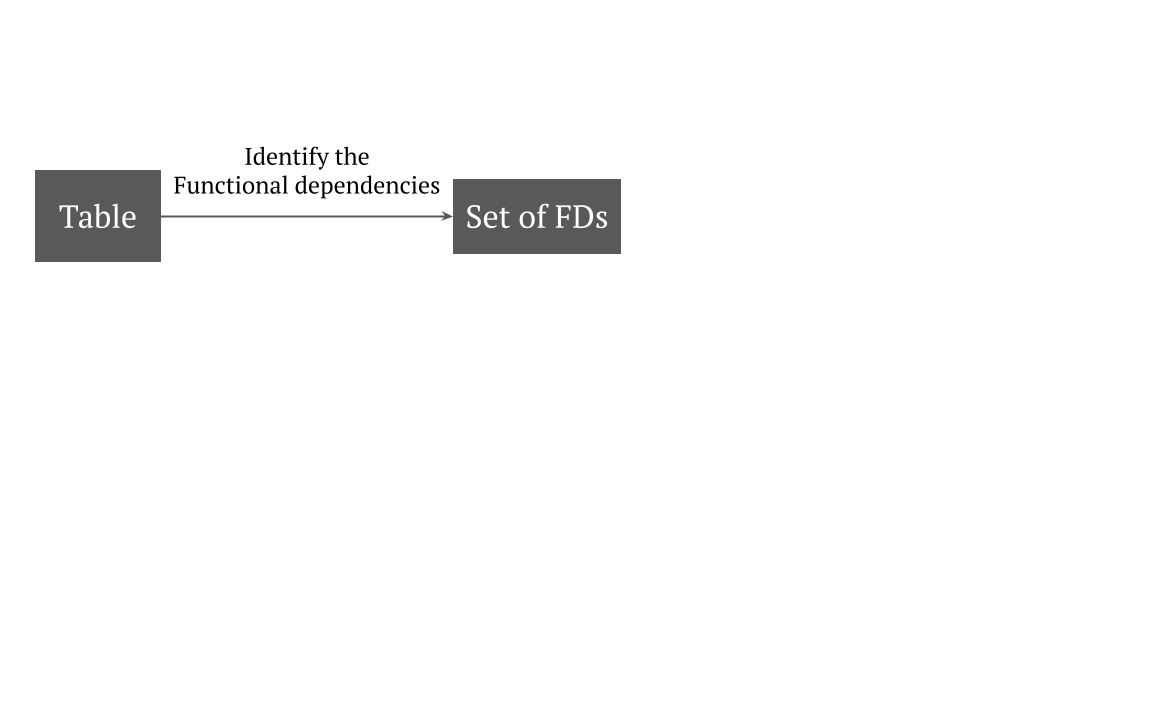
\includegraphics[width = 1\linewidth]{fd_norm_images/02.png}
\end{center}
\end{frame}

\begin{frame}{Overview}
\begin{center}
    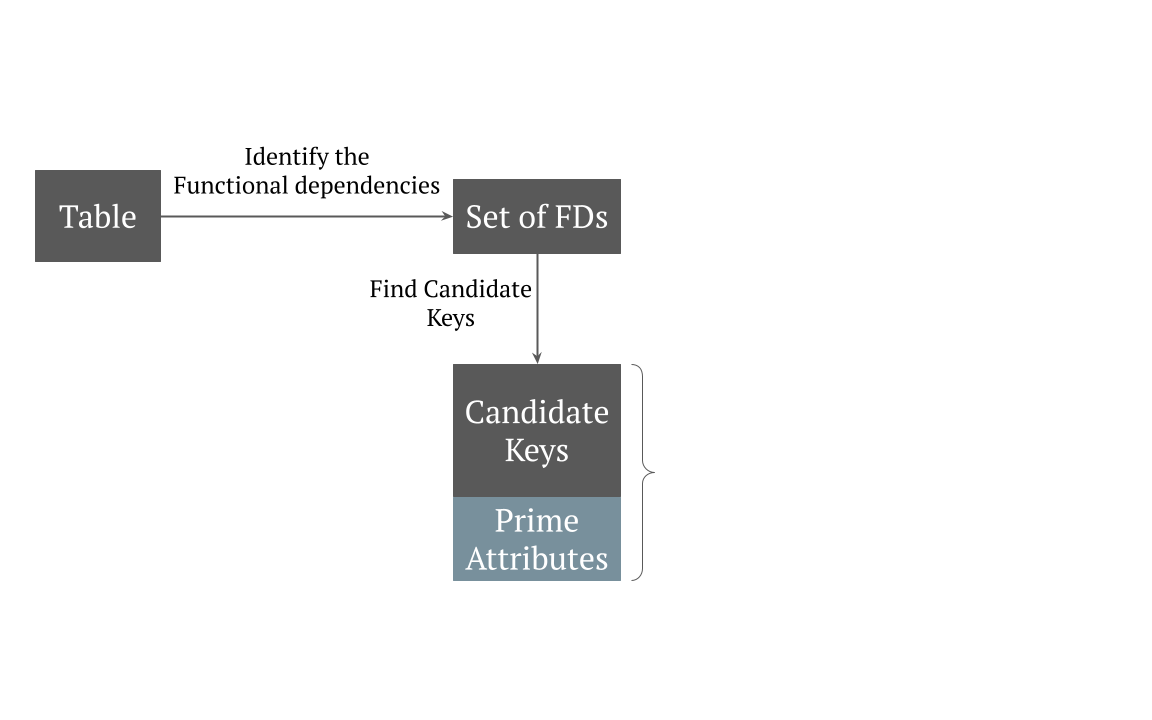
\includegraphics[width = 1\linewidth]{fd_norm_images/03.png}
\end{center}
\end{frame}

\begin{frame}{Overview}
\begin{center}
    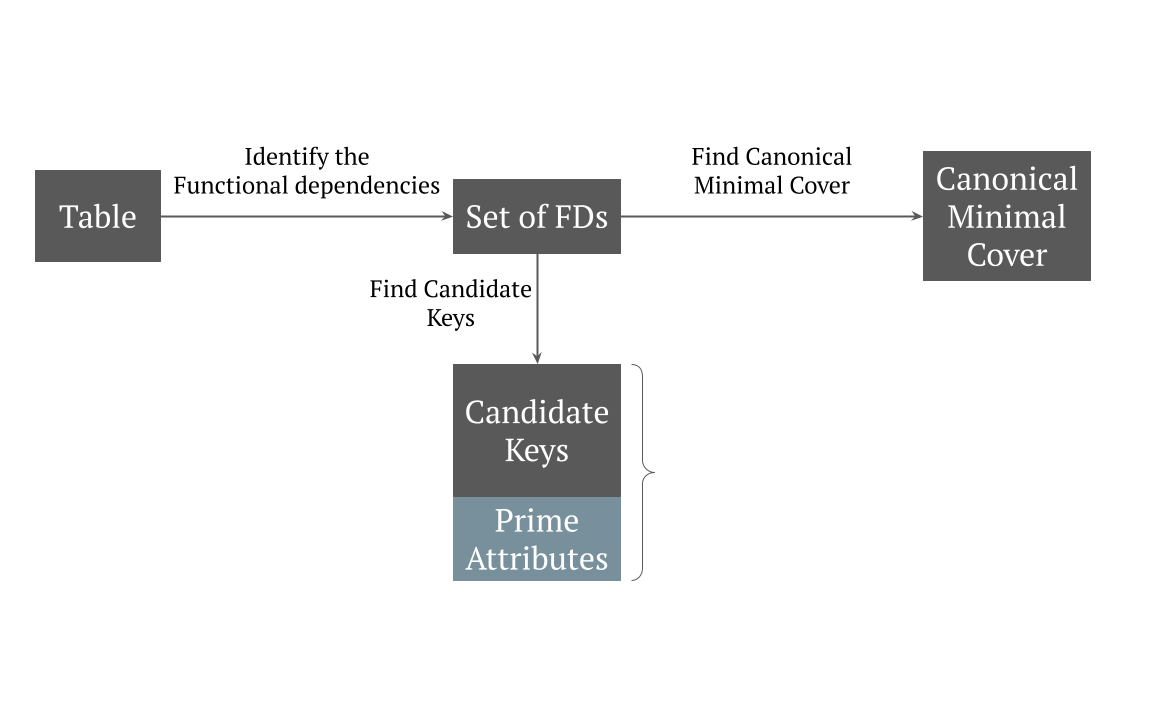
\includegraphics[width = 1\linewidth]{fd_norm_images/04.png}
\end{center}
\end{frame}

\begin{frame}{Overview}
\begin{center}
    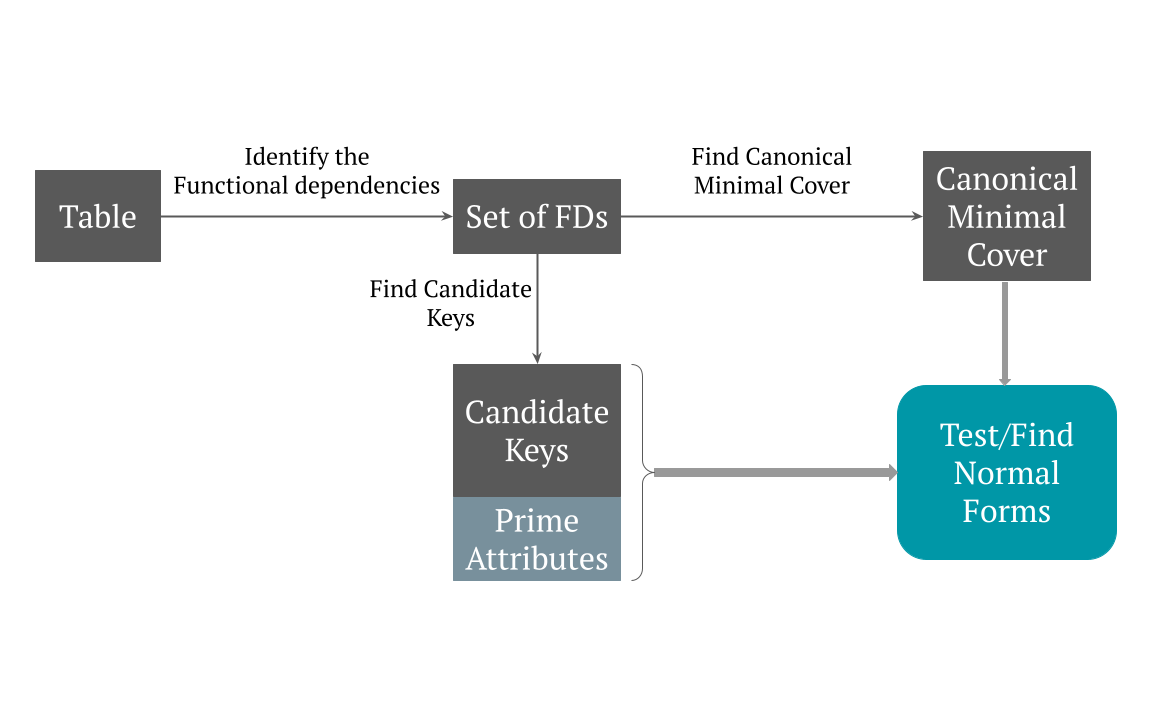
\includegraphics[width = 1\linewidth]{fd_norm_images/05.png}
\end{center}
\end{frame}

\begin{frame}
\begin{center}
Questions?\\
Drop a mail at: pratik.karmakar@u.nus.edu
\end{center}
\end{frame}
\end{document}